\begin{topic}{Application Layer}

The Application Layer provides the interface between the end-user and network communication.

Implementation aspects of network protocols
\begin{itemize}
	\item transport-layer service models
	\item client-server paradigm
\end{itemize}

\end{topic}

\begin{topic}{Network Applications}

Network applications run on \textbf{different end systems} (network edges) and \textbf{communicate over the network.}

Network applications \textbf{do not} run on network cores.

Network applications allow for \textbf{rapid app development and propagation.}

\end{topic}

\begin{topic}{Network Architectures}

\begin{itemize}
	\item Client-server
	\item Peer-to-peer (P2P)
\end{itemize}

\begin{subtopic}{2}
\textbf{Client-server Architecture} is the classical architecture consisting of communication between \textbf{multiple clients} and a \textbf{singular server.}

The server is \textbf{always-on} with a \textbf{fixed address} that \textbf{can be scaled} to multiple devices.

Clients communicate with directly with the server and \textbf{do not need to be always on or have a fixed address.} Clients \textbf{do not communicate with each other.}
\end{subtopic}

\begin{subtopic}{3}
\textbf{Peer-to-peer Architecture} is a form of network communication where clients (now peers) do not connect to an always-on server and instead \textbf{communicate directly with each other.}

Peers request service from other peer and provide service in return to other peers. Think torrents.

Peers are \textbf{intermittently connected and can change addresses.}
\end{subtopic}

\end{topic}

\begin{topic}{Processes}

A \textbf{Process} is a program running within a host.

Inter-process communication is two processes communicating on the same host.

Messages are exchanged by processes communicating on different hosts.

\begin{subtopic}{2-}
\textbf{Client process:} initiates communcation

\textbf{Server process:} waits for communcation from clients
\end{subtopic}

\begin{subtopic}{3-}
\textbf{P2P Applications have both client and server processes}
\end{subtopic}

\end{topic}

\begin{topic}{Sockets}

Processes send and receive messages to and from sockets.

\textbf{Sockets} are connections between host devices.

\end{topic}

\begin{topic}{Addressing Processes}

Processes require \textbf{identifiers} so that messages can be sent back to the correct process.

Each \textbf{host} has a \textbf{32-bit IP address.}

A host can have \textbf{multiple processes} so IP addresses are combined with \textbf{port numbers} as \textbf{identifiers.}

\end{topic}

\begin{topic}{App-Layer Protocol}

App-Layer Protocol defines:
\begin{itemize}
	\item \textbf{type of message} e.g. request, response
	\item \textbf{message syntax:} message fields and encoding
	\item \textbf{message semantics:} meaning of the fields
	\item \textbf{rules:} how processes should send/receive messages
\end{itemize}

\begin{subtopic}{2-}
Open protocols:
\begin{itemize}
	\item defined in \textbf{RFCs}
	\item allows for \textbf{interoperability}
\end{itemize}
\end{subtopic}

\begin{subtopic}{3-}
Proprietary protocols:
\begin{itemize}
	\item normally implemented for a specific proprietary application
\end{itemize}
\end{subtopic}

\end{topic}

\begin{topic}{Transport Service Considerations}

\begin{subtopic}{1-}
\textbf{Data Integrity}
Reliability of data to reach the destination.
Some applications require all data to reach the destination.
\end{subtopic}

\begin{subtopic}{2-}
\textbf{Timing}
Speed transportation takes.
Some applications require fast transportation to work well.
\end{subtopic}

\begin{subtopic}{3-}
\textbf{Throughput}
Amount of data in a transfer.
Some applications require large throughput while others require minimal throughput.
\end{subtopic}

\end{topic}

\begin{topic}{TCP \& UDP}
\begin{multicols}{2}
\textbf{TCP}\\

\begin{itemize}
	\item \textbf{reliable} transport protocol
	\item \textbf{flow control} prevent overwhelming receiver
	\item \textbf{congestion control} prevent overwhelming network
	\item \textbf{no} timing, minimum throughput guarantee, security
	\item \textbf{setup required} connections need to be established
\end{itemize}

\columnbreak
\textbf{UDP}\\

\begin{itemize}
	\item \textbf{unreliable} transport protocol
	\item \textbf{no} flow control, congestion control, timing, throughput guarantee, security, or connection setup
\end{itemize}
\end{multicols}
\end{topic}

\begin{topic}{Secure TCP}

TCP \& UCP connections have \textbf{no encryption.}

\textbf{SSL} connections are encrypted TCP connections.

SSL connections increase \textbf{data integrity} and offer \textbf{end-point authentication.}

SSL is an application layer protocol. Applications use SSL libraries.

\end{topic}

\begin{topic}{Secure TCP}

TCP \& UCP connections have \textbf{no encryption.}

\textbf{SSL} connections are encrypted TCP connections.

SSL connections increase \textbf{data integrity} and offer \textbf{end-point authentication.}

SSL is an application layer protocol. Applications use SSL libraries.

\end{topic}

\begin{topic}{HTTP: Hypertext Transfer Protocol}

Application protocol for websites.

\textbf{Client requests} web objects from server.

\textbf{Server responds} with web objects when requested.

HTTP uses TCP connections (port 80)

HTTP is a \textbf{stateless protocol}. Server does not maintain client information.

\textbf{Persistent HTTP} allows \textbf{multiple objects} per connection. 


\end{topic}

\begin{topic}{Non-persistent HTTP}

\textbf{Non-persistent HTTP} restricts \textbf{one object} per connection.

\begin{enumerate}
	\item Client makes TCP connection to port 80 using a socket
	\item Server accepts incoming TCP connection
	\item Client sends request message over socket to access a resource
	\item Server responds with requested resource
	\item Server closes connection
	\item Client receives requested resource
\end{enumerate}

\end{topic}

\begin{topic}{Non-persistent HTTP Time}

\begin{multicols}{2}
\textbf{RTT:} time for a packet to travel from a client to a server and back.

\textbf{Non-persistent Response Time = } initial RTT + request RTT + file transmission time

\columnbreak
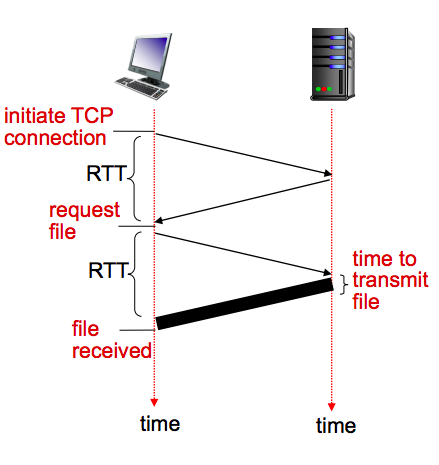
\includegraphics[scale=0.35]{coms3200/images/nonpersistent}
\end{multicols}

\end{topic}

\begin{topic}{Persistent HTTP}

Non-persistent HTTP requires 2 RTTs + OS overheard for each object.

\textbf{Persistent HTTP} leaves connections open allowing for as little as 1 RTT per object.

\end{topic}

\begin{topic}{HTTP Messages}

There are \textbf{request} and \textbf{response} HTTP messages

\begin{subtopic}{2}
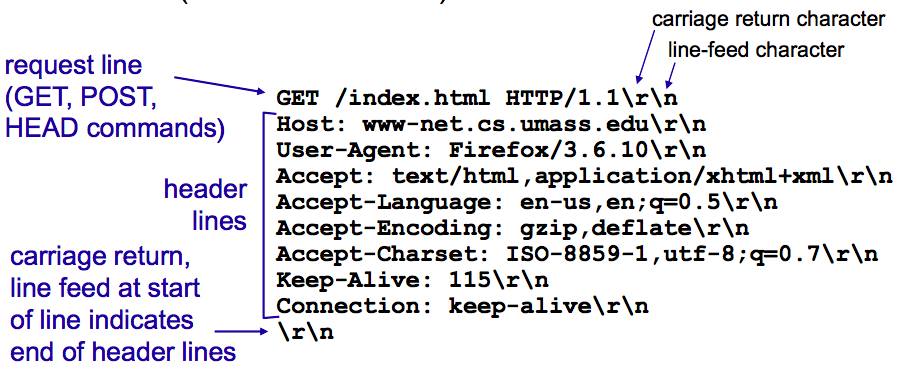
\includegraphics[scale=0.35]{coms3200/images/request}
\end{subtopic}

\begin{subtopic}{3}
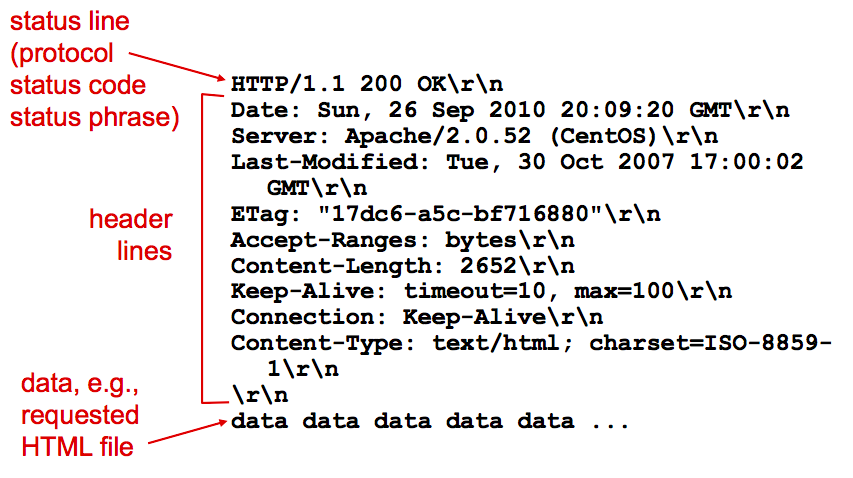
\includegraphics[scale=0.35]{coms3200/images/response}
\end{subtopic}

\begin{subtopic}{4}
\textbf{Method Types}
\begin{multicols}{2}
\textbf{HTTP 1.0 Methods:} GET, POST, HEAD

\textbf{HEAD} asks the server to not send back the requested object.

\columnbreak

\textbf{HTTP 1.1 Methods:} GET, POST, HEAD, PUT, DELETE

\textbf{PUT} uploads object to the given URL

\textbf{DELETE} deletes object at given URL
\end{multicols}
\end{subtopic}

\begin{subtopic}{5}
\textbf{Response Codes}

\begin{itemize}
	\item 200 OK
	\item 301 Moved Permanately
	\item 400 Bad Request
	\item 404 Not Found
	\item 505 HTTP Version Not Supported
\end{itemize}

\end{subtopic}

\end{topic}